Langt de fleste mennesker beskæftiger sig dagligt med SMS'er - dog uden at vide hvad der i virkeligheden sker, når der sendes en SMS. Selv når en mobiltelefon ikke er i brug, sender og modtager den små datapakker til/fra SMS-centeret. Disse data hjælper blandt andet med at lokalisere de basestationer, mobiltelefonen er tættest på.

Når en SMS besked bliver sendt fra en mobiltelefon bliver den i første omgang sendt til mobilcentralen via basestationerne. Når mobilcentralen modtager beskeden bliver den overført til et SMS-center (SMSC). SMS-centeret tager sig af at sende beskeden til den rette modtager, ved at overføre den til den ønskede modtagers SMS-center. Når beskeden når frem til den pågældendes center, bliver den, hvis det er muligt, overført til mobilcentralen der sender beskeden til modtageren. SMS-centeret kan endvidere sende en bekræftelse til afsenderen, når beskeden bliver leveret til modtageren. Et overblik over kommunikationen ses i figur \ref{smsTransm}. Alt dette er muligt via Signaling System no. 7 - som er en protokol suite, der indeholder forskellige protokoller. Protokollerne benyttet af SMS-systemer, befinder sig mere specifikt i SS7 suitens Mobile Application Part (MAP). \cite{Pro_1} \cite{sms_max1}

\noindent
\begin{figure}[hba]
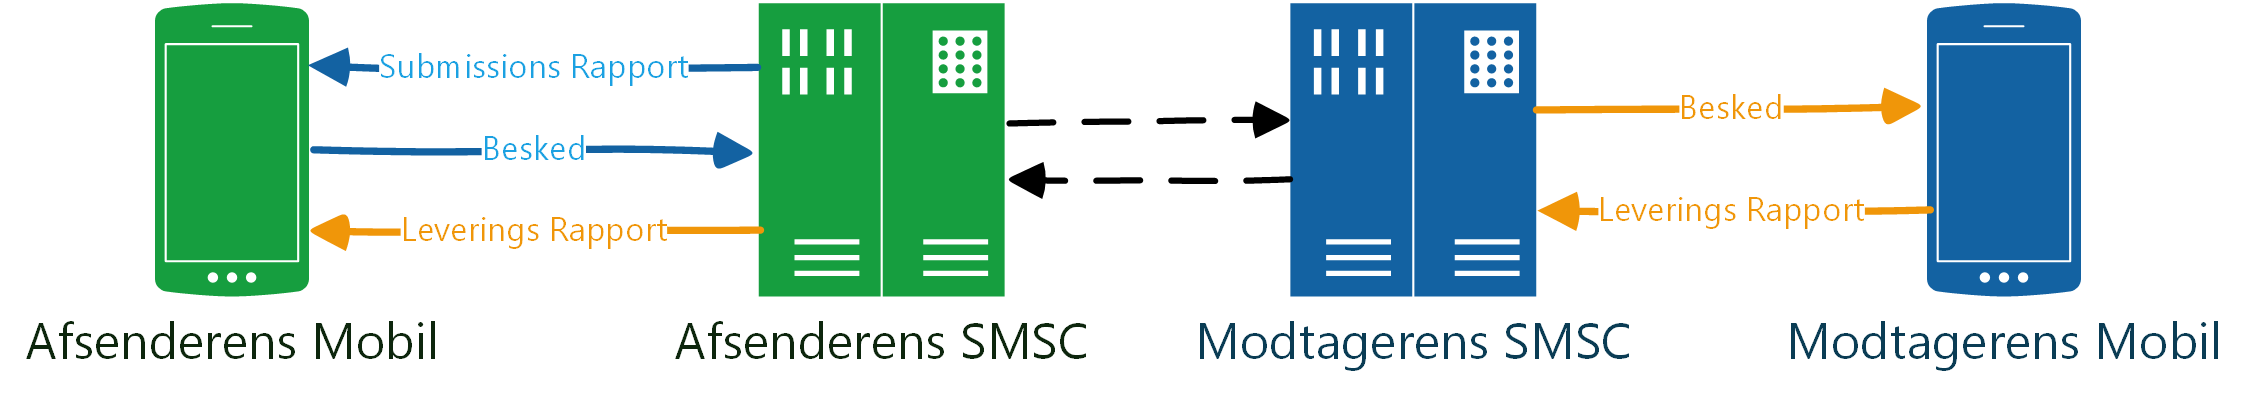
\includegraphics[width=\linewidth]{Billeder/Mobil.png}
\caption {Kommunikationen ved transmission af SMS-beskeder.}
\label{smsTransm}
\end{figure}

Signalerings systemerne i MAP er efter design begrænset til visse størrelser af data. Da man byggede SMS-systemet, talte man tegnene i forskellige beskeder, hvorefter man fandt ud af, at langt de fleste var under 160 tegn. Man mente derfor, at 160 tegn var rigeligt til at rumme de fleste beskeder, hvorved en SMS-beskeds maksimale størrelse blev derfor defineret til 160 tegn. Efter introduktion af udvidede tegnsæt er definitionen præciseret til 140 bytes, eller 1120 bits. \cite{sms_max1} \cite{sms_max2}


Da begrænsningen er defineret i bits, er beskedens maksimale længde afhængig af det anvendte tegnsæt. Det mest almindelige tegnsæt er det grundlæggende 7-bit GSM alfabet. Dette alfabet benytter 7-bits til at symbolisere tegn, hvilket udgør 128 forskellige muligheder. 7-bit GSM alfabetet begrænser derfor en SMS-beskeds længde til 1120/7 bits = 160 tegn. Når der er brug for mere avancerede specialtegn, bruger SMS systemer UCS-2 tegnsættet. Dette tegnsæt benytter 2 okteter - altså 16 bits - til repræsentation af ét tegn. Ved brug af dette tegnsæt mindskes den maksimale længde derfor ned til 1120/16 = 70 tegn. \cite{sms_pdu}

Enhver SMS-besked indeholder også en header\cite{sms_pdu}, som der er afsat plads til udover de 140 okteter. En SMS-header indeholder typisk data som f.eks. afsenderens telefonnummer, længden af beskeden, benyttet tegnsæt og lignende. Hvis en SMS besked bliver længere end grænsen, på det benyttede tegnsæt, bliver beskeden delt op i flere beskeder. Når en besked bliver delt op, skrives der information til fletning af beskeden i headeren - og da der ikke er afsat plads til ekstra header information, bliver der brugt 6 okteter af de oprindelige 140 i beskeden. Dette begrænser længden yderligere til 153 ved 7-bit encoding og 67 ved 16-bit encoding. 
